Here we provide a complete example of how to run the \glsentryfull{qmla} framework, 
    including how to implement a custom \glsentryfull{es}, 
    and generate/interpret analysis.
\par 

First, \emph{fork} the \gls{qmla} codebase from \cite{flynn2021QMLA}
    to a Github user account (referred to as \ttt{username} in \cref{listing:qmla_setup}).
Now, we must download the code base and ensure it runs properly;
    these instructions are implemented via the command line\footnotemark. 
\footnotetext{
    Note: these instructions are tested for Linux and presumed to work on Mac, but untested on Windows. 
    It is likely some of the underlying software (redis servers) can not be installed on Windows,
    so running on \emph{Windows Subsystem for Linux} is advised. 
}

    
\begin{lstlisting}[
    label=listing:qmla_setup,
    caption={QMLA codebase setup. 
    (i) install \ttt{redis};
    (ii) creaet a virtual Python environment for installing \gls{qmla} dependencies without damaging other parts of 
    the user's environment;
    (iii) download the \gls{qmla} codebase from 
        the forked Github repository;
    (iv) install packages upon which \gls{qmla} depends. 
    },
    language=Bash
]
# Install redis (database broker)
sudo apt update
sudo apt install redis-server
 
# make directory for QMLA
cd
mkdir qmla_test
cd qmla_test

# make Python virtual environment for QMLA
# note: change Python3.6 to desired version
sudo apt-get install python3.6-venv 
python3.6 -m venv qmla-env    
source qmla-env/bin/activate

# Download QMLA
git clone --depth 1 https://github.com/username/QMLA.git # REPLACE username

# Install dependencies
cd QMLA 
pip install -r requirements.txt 
\end{lstlisting}

Note there may be a problem with some packages in the \ttt{requirements.txt} arising from the attempt to install them all through
a single call to \ttt{pip install}. 
Ensure these are all installed before proceeding. 
\par 

When all of the requirements are installed, test that the framework runs. 
\gls{qmla} uses \ttt{redis} databases to store intermittent data:
    we must manually initialise the database. 
Run the following 
    (note: here we list \ttt{redis-4.0.8}, but this must be corrected to reflect the 
    version installed on the user's machine in the above setup section):
\begin{lstlisting}[
    label=listing:athlete_class,
    caption={Launch redis database},
    language=Bash
]
~/redis-4.0.8/src/redis-server
\end{lstlisting}

which should give something like \cref{fig:terminal_redis}.
\begin{figure}[h!]
    \begin{center}
        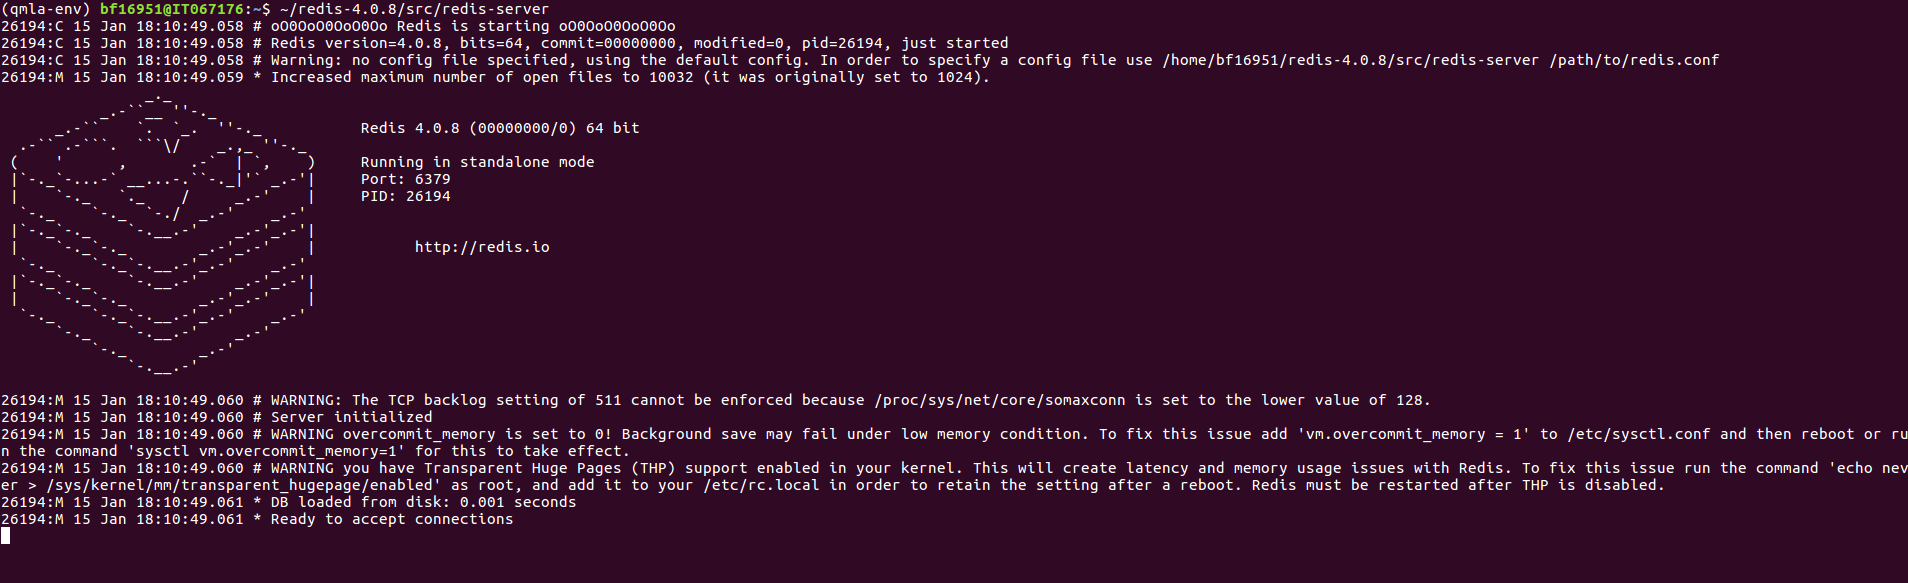
\includegraphics[width=0.9\textwidth]{appendix/figures/terminal_redis.png}
    \end{center}
    \caption[Terminal running redis-server]{Terminal running \ttt{redis-server}.}
    \label{fig:terminal_redis}
\end{figure}
\par 

In a text editor, open \ttt{qmla\_test/QMLA/launch/local\_launch.sh}; 
    here we will ensure that we are running the \gls{qhl} algorithm, 
    with 5 experiments and 20 particles, on the \gls{es} named \ttt{TestInstall}.
Ensure the first few lines of \ttt{local\_launch.sh} read:

\begin{lstlisting}[
    label=listing:local_launch,
    caption={\ttt{local\_launch} script},
    language=Bash
]
#!/bin/bash

##### -------------------------------------------------- #####
# QMLA run configuration
##### -------------------------------------------------- #####
num_instances=2 # number of instances in run
run_qhl=0 # perform QHL on known (true) model
run_qhl_multi_model=0 # perform QHL for defined list of models
experiments=2 # number of experiments
particles=10 # number of particles
plot_level=5


##### -------------------------------------------------- #####
# Choose an exploration strategy 
# This will determine how QMLA proceeds. 
##### -------------------------------------------------- #####
exploration_strategy="TestInstall"
\end{lstlisting}    

Now we can run 
Ensure the terminal running redis is kept active, and open a separate terminal window. 
We must activate the Python virtual environment configured for \gls{qmla}, 
which we set up in \cref{listing:qmla_setup}. 
Then, we navigate to the \gls{qmla} directory, and launch:
\begin{lstlisting}[
    label=listing:launch_example,
    caption={Launch QMLA},
    language=Bash
]

# activate the QMLA Python virtual environment 
source qmla_test/qmla-env/bin/activate

# move to the QMLA directory 
cd qmla_test/QMLA
# Run QMLA
cd launch   
./local_launch.sh

\end{lstlisting}

There may be numerous warnings, but they should not affect whether \gls{qmla} has succeeded; 
    \gls{qmla} will \ttt{raise} any significant error. 
Assuming the run has completed successfully, \gls{qmla} stores the run's results in a subdirectory
    named by the date and time it was started.  
For example, if the run was initialised on January $1^{st}$ at 01:23, navigate to the corresponding directory by

\begin{lstlisting}[
    label=listing:results_directory,
    caption={QMLA results directory},
    language=Bash
]
cd results/Jan_01/01_23
\end{lstlisting}

For now it is sufficient to notice that the code has run successfully:
    it should have generated (in \ttt{results/Jan\_01/01\_23}) files like \ttt{storage\_001.p} and \ttt{results\_001.p}.

\section{Custom \glsentrylong{es}}

Next, we design a basic \gls{es}, for the purpose of demonstrating how to run the algorithm.
\glspl{es} are placed in the directory \ttt{qmla/exploration\_strategies}. 
To make a new one, navigate to the exploration strategies directory, 
make a new subdirectory, and copy the template file. 

\begin{lstlisting}[
    label=listing:athlete_class,
    caption={QMLA codebase setup},
    language=Bash
]

cd ~/qmla_test/QMLA/exploration_strategies/
mkdir custom_es

# Copy template file into example
cp template.py custom_es/example.py
cd custom_es

\end{lstlisting}

Ensure \gls{qmla} will know where to find the \gls{es} by importing everything from the custom \gls{es} 
    directory into to the main \ttt{exploration\_strategy} module. 
Then, in the \ttt{custom\_es} directory, make a file called \ttt{\_\_init\_\_.py} which imports the new \gls{es}
    from the \ttt{example.py} file. 
To add any further \glspl{es} inside the directory \ttt{custom\_es}, include them in the custom \ttt{\_\_init\_\_.py},
    and they will automatically be available to \gls{qmla}.

\begin{lstlisting}[
    label=listing:importing_es,
    caption={Providing custom exploration strategy to QMLA},
    language=Python
]

# inside qmla/exploration_strategies/custom_es
#  __init__.py    
from qmla.exploration_strategies.custom_es.example import *

# inside qmla/exploration_strategies, add to the existing
# __init__.py 
from qmla.exploration_strategies.custom_es import *

\end{lstlisting}

Now, change the structure (and name) of the \gls{es} inside \ttt{custom\_es/example.py}. 
Say we wish to target the true model 
\begin{equation}
    \label{eqn:example_es_true_ham}
    \begin{split}
        \al &= \irow{ \alpha_{1,2} & \alpha_{2,3} & \alpha_{3,4}} \\
        \terms &= \icol{ \sz^1 \otimes \sz^2 \\ \sz^2 \otimes \sz^3  \\ \sz^3 \otimes \sz^4 } \\
        \Longrightarrow \ho &= \sz^{(1,2)} \sz^{(2,3)} \sz^{(3,4)} \\
    \end{split}
\end{equation}

\gls{qmla} interprets models as strings, where terms are separated by \ttt{+}, and parameters are implicit. 
So the target model in \cref{eqn:example_es_true_ham} will be given by 
$$ \ttt{pauliSet\_1J2\_zJz\_d4+pauliSet\_2J3\_zJz\_d4+pauliSet\_3J4\_zJz\_d4}. $$

Adapting the template \gls{es} slightly, we can define a model generation strategy with a small number of hard coded 
    candidate models introduced at the first branch of the \glsentrylong{et}. 
We will also set the parameters of the terms which are present in $\ho$, as well as the range in which to search parameters.
Keeping the \ttt{import}s at the top of the \ttt{example.py}, rewrite the \gls{es} as: 

\begin{lstlisting}[
    label=listing:basic_es,
    caption={ExampleBasic exploration strategy.},
    language=Python
]
class ExampleBasic(
    exploration_strategy.ExplorationStrategy
):

    def __init__(
        self,
        exploration_rules,
        true_model=None,
        **kwargs
    ):
        self.true_model = 'pauliSet_1J2_zJz_d4+pauliSet_2J3_zJz_d4+pauliSet_3J4_zJz_d4'
        super().__init__(
            exploration_rules=exploration_rules,
            true_model=self.true_model,
            **kwargs
        )

        self.initial_models = None
        self.true_model_terms_params = {
            'pauliSet_1J2_zJz_d4' : 2.5,
            'pauliSet_2J3_zJz_d4' : 7.5,
            'pauliSet_3J4_zJz_d4' : 3.5,
        }
        self.tree_completed_initially = True
        self.min_param = 0
        self.max_param = 10

    def generate_models(self, **kwargs):

        self.log_print(["Generating models; spawn step {}".format(self.spawn_step)])
        if self.spawn_step == 0:
            # chains up to 4 sites
            new_models = [
                'pauliSet_1J2_zJz_d4',
                'pauliSet_1J2_zJz_d4+pauliSet_2J3_zJz_d4',
                'pauliSet_1J2_zJz_d4+pauliSet_2J3_zJz_d4+pauliSet_3J4_zJz_d4',
            ]
            self.spawn_stage.append('Complete')

        return new_models

\end{lstlisting}


To run\footnotemark \ the example \gls{es} for a meaningful tests, 
    return to the \ttt{local\_launch} of \cref{listing:local_launch}, 
    but change some of the settings:
\begin{lstlisting}[
    label=listing:example_es_qhl_run,
    caption={\ttt{local\_launch} configuration for QHL.},
    language=Bash
]
prt=2000
exp=500
run_qhl=1
exploration_strategy=ExampleBasic
\end{lstlisting}

Run locally again as in \cref{listing:launch_example};
    then move to the results directory as in \cref{listing:results_directory}. 
\footnotetext{
    Note this will take up to 15 minutes to run. 
    This can be reduced by lowering the values of \ttt{prt}, \ttt{exp}, 
    which is sufficient for testing but note that the outcomes will be less effective 
    than those presented in the figures of this section.
}
\par 


\section{Analysis}
\gls{qmla} stores results and generates plots
    over the entire range of the algorithm\footnotemark, i.e. the \gls{run}, \gls{instance} and models. 
\footnotetext{Recall that a single implementation of \gls{qmla} is called an \gls{instance},    
    while a series of instances -- which share the same target model -- is called the \gls{run}.}
The depth of analysis performed automatically is set by the user control \ttt{plot\_level} in \ttt{local\_launch.sh};
    for \ttt{plot\_level=1}, only the most crucial figures are generated, while \ttt{\plot\_level=6} generates plots for every individual 
    model considered. 
For model searches across large model spaces and/or considering many candidates,
    excessive plotting can cause considerable slow-down, so users should be careful to generate plots only 
    to the degree they will be useful. 
Next we show some examples of the available plots. 
\par 

\subsection{Model analysis}

We have just run \glsentryfull{qhl} for the model in \cref{eqn:example_es_true_ham} for a single instance, 
    using a reasonable number of particles and experiments, so we expect to have trained the model well. 
Instance-level results are stored (e.g. for the instance with \ttt{qmla\_id=1}) in \ttt{Jan\_01/01\_23/instances/qmla\_1}.
Individual models' insights can be found in \ttt{model\_training}, 
    e.g. the model's \ttt{learning\_summary} \cref{fig:qmla_learning_summary}, and \ttt{dynamics} in \cref{fig:qmla_model_dynamics}.
\par 

\begin{figure}[H]
    \begin{center}
    \subfloat[]{
        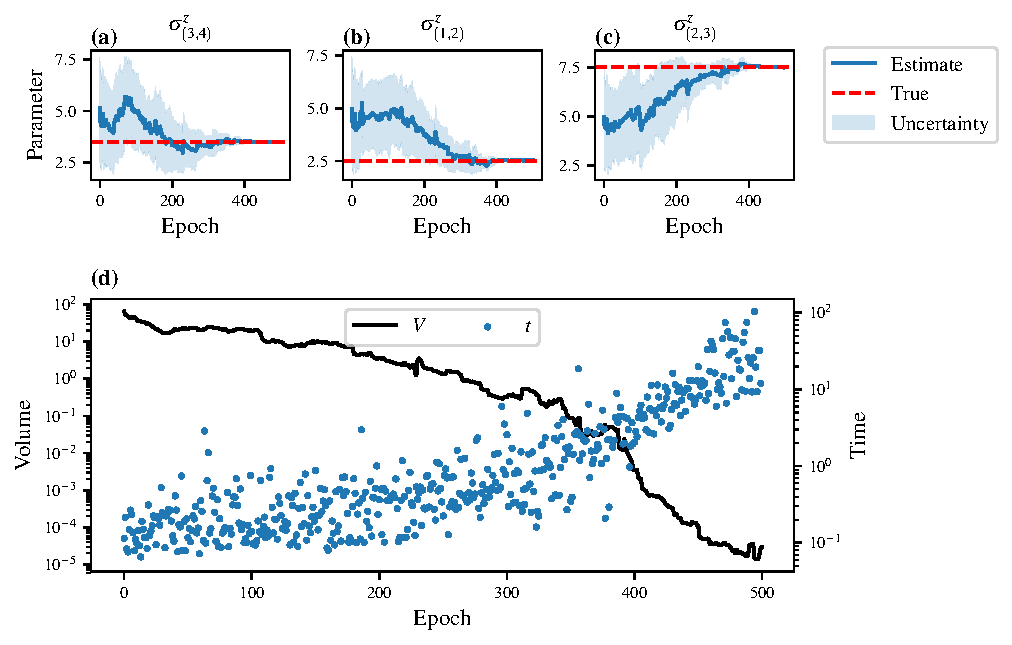
\includegraphics[width=0.75\textwidth]{qmla_run_data/Jan_17/18_04/instances/qmla_1/model_training/learning_summary_1.pdf}
        \label{fig:qmla_learning_summary}
    }
    \qquad
    \subfloat[]{
        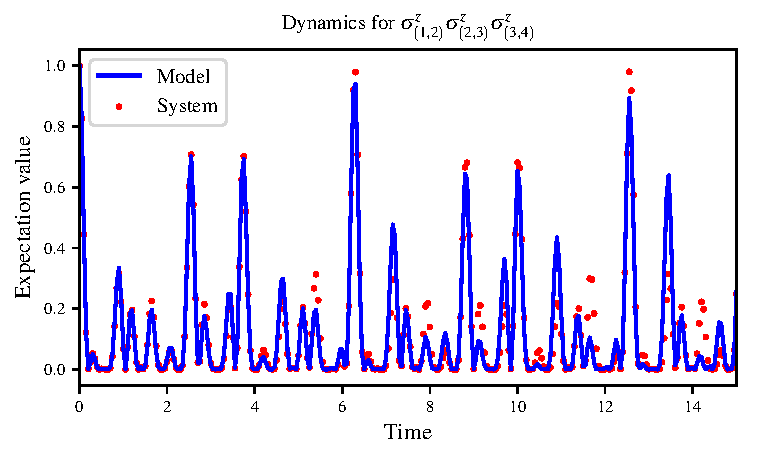
\includegraphics[width=0.75\textwidth]{qmla_run_data/Jan_17/18_04/instances/qmla_1/model_training/dynamics_1.pdf}
        \label{fig:qmla_model_dynamics}
    }
    \end{center}
    \caption[Model analysis plots]{
        Model analysis plots, stored in (for example) \ttt{Jan\_01/01\_23/instances/qmla\_1/model\_training}. 
        \textbf{a} \ttt{learning\_summary\_1}. 
        Displays the outcome of \gls{qhl} for the given model:
        Subfigures (a)-(c) show the estimates of the parameters; 
        (d) shows the total parameterisation volume against experiments trained upon, 
        along with the evolution times used for those experiments. 
        \textbf{(b)} \ttt{dynamics\_1} The model's attempt at reproducing dynamics from $\ho$. 
    }
    \label{fig:model_analysis}
\end{figure}

\subsection{\Gls{instance} analysis}
Now we can run the full \gls{qmla} algorithm, i.e. train several models 
    and determine the most suitable. 
\gls{qmla} will call the \ttt{generate\_models} method of the \ttt{ExampleBasic} \gls{es},
    set in \cref{listing:basic_es}, which tells \gls{qmla} to construct three models
    on the first branch, then terminate the search.
Here we need to train and compare all models so it takes considerably longer to run:
    the purpose of testing, we reduce the resources so the entire algorithm runs in about 15 minutes.
Some applications will require significantly more resources to learn effectively.
In realistic cases, these processes are run in parallel, as we will cover in \cref{apdx:paralllel_processing}.
\par 

Reconfigure a subset of the settings in the \ttt{local\_launch.sh} script (\cref{listing:local_launch}) and run it again:
\begin{lstlisting}[
    label=listing:example_es_qhl_run,
    caption={\ttt{local\_launch} configuration for QMLA.},
    language=Bash
]
exp=250
prt=1000
run_qhl=0
exploration_strategy=ExampleBasic
\end{lstlisting}

\par 

In the corresponding results directory, navigate to \ttt{instances/qmla\_1}, where instance level analysis are available. 

\begin{lstlisting}[
    label=listing:instance_results,
    caption={Navigating to instance results.},
    language=Bash
]
cd results/Jan_01/01_23/instances/qmla_1
\end{lstlisting}

Figures of interest here show the composition of the models (\cref{fig:qmla_model_composition}), 
    as well as the \glsentrylongpl{bf} between candidates (\cref{fig:qmla_bayes_factors}). 
Individual model comparisons -- i.e. \glsentryfull{bf} -- 
    are shown in \cref{fig:qmla_bayes_factor_comparison}, 
    with the dynamics of all candidates shown in \cref{fig:qmla_branch_dynamics}. 
The probes used during the training of all candidates are also plotted  (\cref{fig:qmla_training_probes}).

\begin{figure}[H]
    % TODO use Jan_18/13_15 without rescaling images
    \begin{center}
        \subfloat[]{
            \includegraphics{qmla_run_data/Jan_18/14_36/instances/qmla_10/composition_of_models.pdf}
            \label{fig:qmla_model_composition}
        }
        \qquad
        \subfloat[]{
            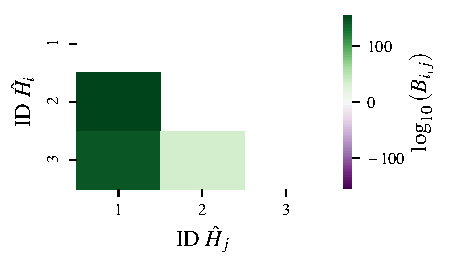
\includegraphics{qmla_run_data/Jan_18/14_36/instances/qmla_10/bayes_factors.pdf}
            \label{fig:qmla_bayes_factors}
        }
        \qquad
        \subfloat[]{
            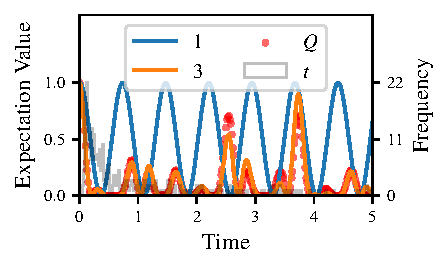
\includegraphics{qmla_run_data/Jan_18/14_36/instances/qmla_10/comparisons/BF_1_3.pdf}
            \label{fig:qmla_bayes_factor_comparison}
        }
        \qquad
        \subfloat[]{
            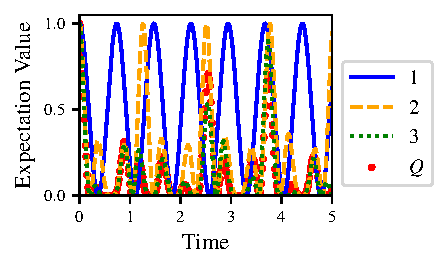
\includegraphics{qmla_run_data/Jan_18/14_36/instances/qmla_10/branches/dynamics_branch_1.pdf}
            \label{fig:qmla_branch_dynamics}
        }
        \qquad
        \subfloat[]{
            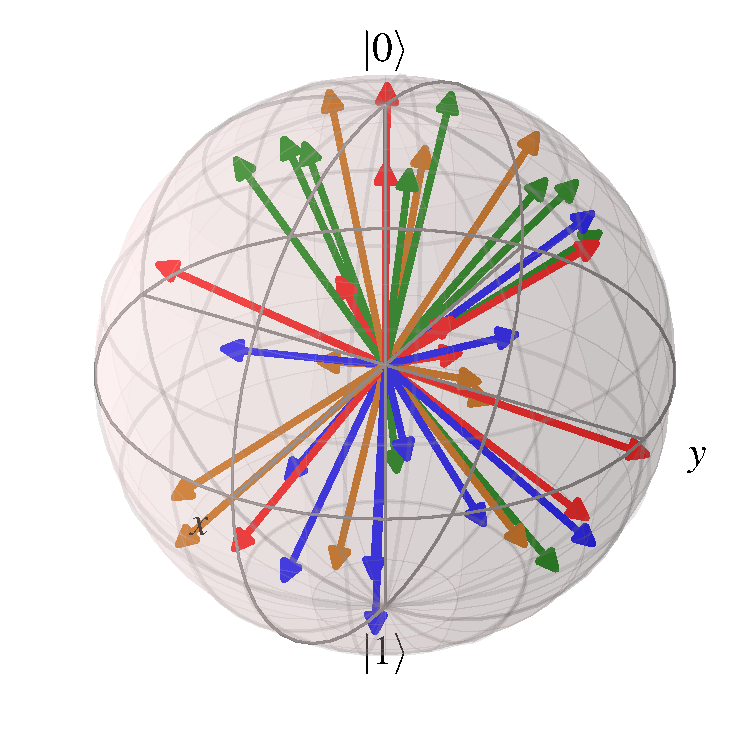
\includegraphics[width=0.25\textwidth]{qmla_run_data/Jan_18/14_36/instances/qmla_10/probes_bloch_sphere.pdf}
            \label{fig:qmla_training_probes}
        }
    \end{center}
    \caption[Instance plots]{
        \gls{qmla} plots; found within instance directory e.g. \ttt{Jan\_01/01\_23/instances/qmla\_1}, 
        and its subdirectories. 
        \textbf{(a)} \ttt{composition\_of\_models}: constituent terms of all considered models, indexed by their model IDs.
        Here model 3 is $\ho$. 
        \textbf{(b)} \ttt{bayes\_factors}: \glsentryfull{bf} comparisons between all models. 
        \glspl{bf} are read as $B_{i,j}$ where $i$ is the model with lower ID, 
            e.g. $B_{1,2}$ rather than $B_{2,1}$. 
            Thus $B_{ij} > 0 \ (<0)$ indicates $\hat{H}_i$ \ ($\hat{H}_j$), i.e. the model on the $y$-axis ($x$-axis) 
            is the stronger model.
        \textbf{(c)} \ttt{comparisons/BF\_1\_3}: direct comparison between models with IDs 1 and 3, 
            showing their reproduction of the system dynamics (red dots, $Q$), 
            as well as the times (experiments) against which the \gls{bf} was calculated. 
        \textbf{(d)} \ttt{branches/dynamics\_branch\_1}: dynamics of all models considered on the branch
        compared with system dynamics (red dots, $Q$). 
        \textbf{(e)} \ttt{probes\_bloch\_sphere}: probes used for training models in this instance (only showing 1-qubit versions).
    }
    \label{fig:instance_plots}
\end{figure}

\subsection{\Gls{run} analysis}
Considering a number of \glspl{instance} together is a \emph{\gls{run}}. 
In general, this is the level of analysis of most interest: 
    an individual instance is liable to errors due to the probabilistic nature of 
    the model training and generation subroutines. 
On average, however, we expect those elements to perform well, 
    so across a significant number of instances, we expect the average outcomes to be meaningful. 
\par 

Each results directory has an \ttt{analyse.sh} script to generate plots at the \gls{run} level. 
\begin{lstlisting}[
    label=listing:analysing_run,
    caption={Analysing QMLA run.},
    language=Bash
]
cd results/Jan_01/01_23
./analyse.sh
\end{lstlisting}

Run level analysis are held in the main results directory and several sub-directories created by the \ttt{analyse} script. 
Here, we recommend running a number of instances with very few resources so that the test finishes quickly\footnote{This run will take about ten minutes}. 
The results will therefore be meaningless, but allow fo elucidation of the resultant plots. 
First, reconfigure some settings of \cref{listing:local_launch} and launch again.
\begin{lstlisting}[
    label=listing:example_es_qhl_run,
    caption={\ttt{local\_launch} configuration for QMLA run.},
    language=Bash
]
num_instances=10
exp=20
prt=100
run_qhl=0
exploration_strategy=ExampleBasic
\end{lstlisting}
\par 

Some of the generated analysis are shown in \crefrange{fig:run_plots}{fig:run_dynamics}. 
The number of instances for each model, i.e. their \emph{\glspl{win rate}} are given in \cref{fig:qmla_win_rates}.
The \emph{top models}, i.e. those with highest win rates, analysed further: 
    the average parameter estimation progression for $\ho$ -- including only the instances where $\ho$ was deemed champion --
    are shown in \cref{fig:champ_param_progression}.
Irrespecitve of the champion models, the rate with which each term is found in the champion model ($\hat{t} \in \hp$)
    indicates the likelihood that the term is really present;
    these rates -- along with the parameter values learned -- are shown in \cref{fig:qmla_branch_dynamics}.
The champion model from each instance can attempt to reproduce system dynamics: 
    we group together these reproductions for each model in \cref{fig:run_dynamics}. 

\begin{figure}[H]
    \begin{center}
        \subfloat[]{
            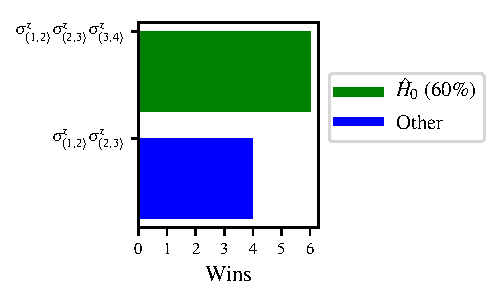
\includegraphics{qmla_run_data/Jan_17/22_27/performance/model_wins.pdf}
            \label{fig:qmla_win_rates}
        }
        \qquad
        \subfloat[]{
            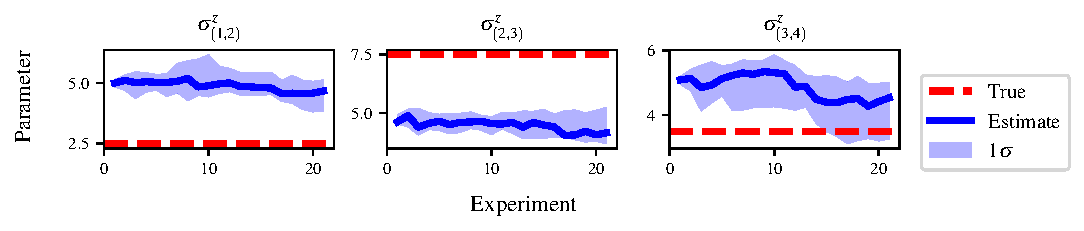
\includegraphics{qmla_run_data/Jan_17/22_27/champion_models/params_pauliSet_1J2_zJz_d4+pauliSet_2J3_zJz_d4+pauliSet_3J4_zJz_d4.pdf}
            \label{fig:champ_param_progression}
        }
        \qquad
        \subfloat[]{
            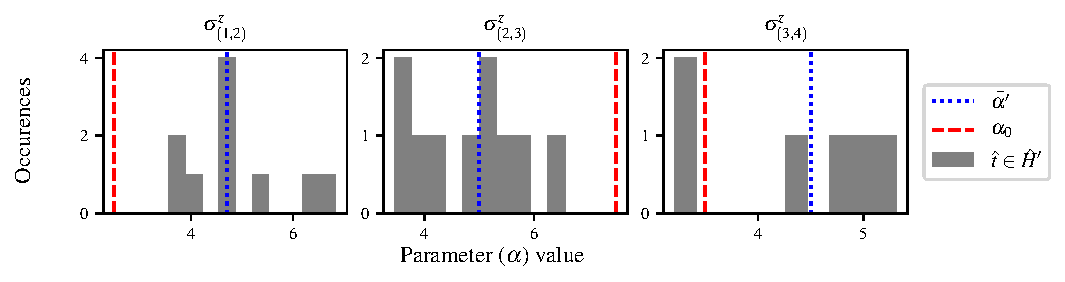
\includegraphics{qmla_run_data/Jan_17/22_27/champion_models/terms_and_params.pdf}
            \label{fig:qmla_branch_dynamics}
        }
    \end{center}
    \caption[Run plots]{
        \gls{qmla} run plots; found within run directory e.g. \ttt{Jan\_01/01\_23/}. 
        \textbf{(a)} \ttt{performace/model\_wins}: number of instance wins achieved by each model. 
        \textbf{(b)} \ttt{champion\_models/params\_params\_pauliSet\_1J2\_zJz\_d4+pauliSet\_2J3\_zJz\_d4+pauliSet\_3J4\_zJz\_d4}: 
            parameter estimation progression for the true model, only for the instances where it was deemed champion. 
        \textbf{(c)} \ttt{champion\_models/terms\_and\_params}: 
            histogram of parameter values found for each term which appears in any champion model,
            with the true parameter ($\alpha_0$) in red and the median learned parameter ($\bar{\alpha}^{\prime}$) in blue.
    }
    \label{fig:run_plots}
\end{figure}

\begin{figure}[H]
    \begin{center}
        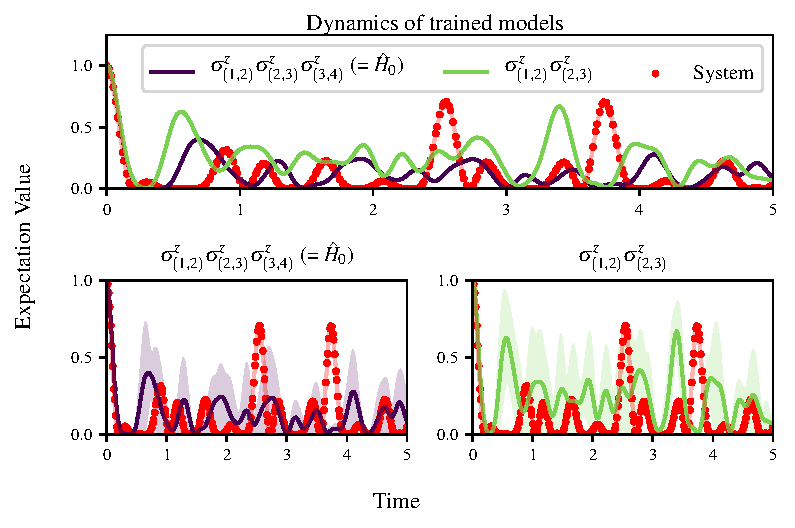
\includegraphics{qmla_run_data/Jan_17/22_27/performance/dynamics.pdf}
    \end{center}
    \caption[Run plot: dynamics]{
        Run plot \ttt{performace/dynamics}: median dynamics of the champion models. 
        The models which won most instances are shown together in the top panel, 
        and individually in the lower panels. 
        The median dynamics from the models' learnings in its winning instances are shown, 
        with the shaded region indicating the 66\% confidence region. 
    }
    \label{fig:run_dynamics}
\end{figure}



\section{Parallel implementation}
We provide utility to run \gls{qmla} on parallel processes. 
Individual models' training can run in parallel, as well as the calculation of \gls{bf} between models. 
The provided script is designed for \gls{pbs} job scheduler running on a compute cluster. 
It will require a few adjustments to match the system being used. 
Overall, though, it has mostly a similar structure as the \ttt{local\_launch.sh} script used above. 
\par 

\gls{qmla} must be downloaded on the compute cluster as in \cref{listing:qmla_setup};
    this can be a new fork of the repository, 
    though it is sensible to test installation locally as described in this chapter so far, 
    then \emph{push} that version, including the new \gls{es}, to Github, 
    and cloning the latest version.
It is again advisable to create a Python virtual environment in order to isolate \gls{qmla} 
    and its dependencies\footnote{Indeed it is sensible to do this for any Python development project.}.
Open the parallel launch script, \ttt{QMLA/launch/parallel\_launch.sh}, and prepare the first few lines as 

\begin{lstlisting}[
    label=listing:parallel_launch,
    caption={\ttt{parallel\_launch} script},
    language=Bash
]
#!/bin/bash

##### -------------------------------------------------- #####
# QMLA run configuration
##### -------------------------------------------------- #####
num_instances=10 # number of instances in run
run_qhl=0 # perform QHL on known (true) model
run_qhl_multi_model=0 # perform QHL for defined list of models
experiments=250
particles=1000
plot_level=5


##### -------------------------------------------------- #####
# Choose an exploration strategy 
# This will determine how QMLA proceeds. 
##### -------------------------------------------------- #####
exploration_strategy="ExampleBasic"
\end{lstlisting}    

\par 

When submitting jobs to schedulers like \gls{pbs}, we must specify the time required, 
    so that it can determine a fair distribution of resources among users. 
We must therefore \emph{estimate} the time it will take for an instance to complete:
    clearly this is strongly dependent on the numbers of experiments ($\Ne$) and particles ($\Np$), 
    and the number of models which must be trained. 
\gls{qmla} attempts to determine a reasonable time to request based on the \ttt{max\_num\_models\_by\_shape}
    attribute of the \gls{es}, by calling \ttt{QMLA/scripts/time\_required\_calculation.py}. 
In practice, this can be difficult to set perfectly,
    so the \ttt{timing\_insurance\_factor} attribute of the \gls{es} can be used to correct 
    for heavily over- or under-estimated time requests. 
Instances are run in parallel, and each instance trains/compares models in parallel. 
The number of processes to request, $N_c$ for each instance is set as \ttt{num\_processes\_to\_parallelise\_over} 
        in the \gls{es}.
Then, if there are $N_r$ instances in the run, we will be requesting the job scheduler to admit 
    $N_r$ distinct jobs, each requiring $N_c$ processes, for the time specified. 

\par 

The \ttt{parallel\_launch} script works together with \ttt{launch/run\_single\_qmla\_instance.sh}, 
    though note a number of steps in the latter are configured to the cluster and may need to be adapted. 
In particular, the first command is used to load the redis utility, and later lines are used to initialise a 
redis server. 
These commands will probably not work with most machines, so must be configured to achieve those steps. 


\begin{lstlisting}[
    label=listing:instace_script,
    caption={\ttt{run\_single\_qmla\_instance} script},
    language=Bash
]

module load tools/redis-4.0.8

... 

SERVER_HOST=$(head -1 "$PBS_NODEFILE")
let REDIS_PORT="6300 + $QMLA_ID"

cd $LIBRARY_DIR
redis-server RedisDatabaseConfig.conf --protected-mode no --port $REDIS_PORT & 
redis-cli -p $REDIS_PORT flushall

\end{lstlisting}

When the modifications are finished, 
    \gls{qmla} can be launched in parallel similarly to the local version: 

\begin{lstlisting}[
    label=listing:instace_script,
    caption={\ttt{run\_single\_qmla\_instance} script},
    language=Bash
]
source qmla_test/qmla-env/bin/activate

cd qmla_test/QMLA/launch
./parallel_launch.sh

\end{lstlisting}
\par 

Jobs are likely to queue for some time, depending on the demands on the job scheduler. 
When all jobs have finished, results are stored as in the local case, 
    in \ttt{QMLA/launch/results/Jan\_01/01\_23},
    where \ttt{analyse.sh} can be used to generate a series of automatic analyses. 
\par 

\section{Customising \glsentrylongpl{es}}
User interaction with the \gls{qmla} codebase should be achieveable primarily through the \glsentryfull{es} framework. 
Throughout the algorithm(s) available, \gls{qmla} calls upon the \gls{es} before determining how to proceed. 
The usual mechanism through which the actions of \gls{qmla} are directed, 
    is to set attributes of the \gls{es} class:
    the complete set of influential attributes are available at \cite{qmla_docs}. 

\par 
\gls{qmla} directly uses several methods of the \gls{es} class, 
    all of which can be overwritten in the course of customising an \gls{es}. 
Most such methods need not be replaced, however, with the exception of \ttt{generate\_models}, 
    which is the most important aspect of any \gls{es}: 
    it determines which models are built and tested by \gls{qmla}. 
This method allows the user to impose any logic desired in constructing models;
    it is called after the completion of every branch of the  \glsentrylong{et} on the \gls{es}. 
\par 

\subsection{Greedy search}sec:greedy_search

A first non-trivial \gls{es} is to build models greedily from a set of \emph{primitive} terms, $\termset = \{ \hat{t} \} $. 
New models are constructed by combining the previous branch champion with each of the remaining, unused terms. 
The process is repeated until no terms remain. 

\begin{figure}[H]
    \begin{center}
        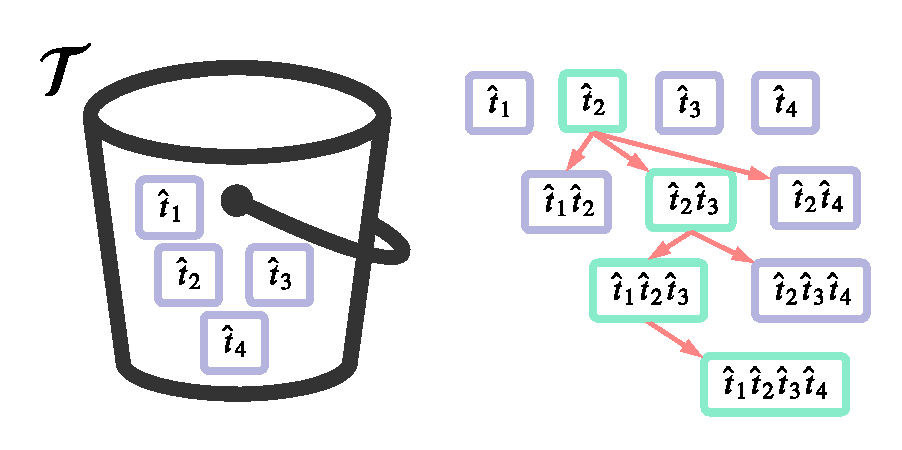
\includegraphics[scale=0.75]{appendix/figures/greedy_exploration_strategy.pdf}
    \end{center}
    \caption[
        Greedy \glsentrylong{es}]{Greedy \glsentrylong{es}.
        \textbf{Left}, a set of primitive terms, $\termset$, are defined in advance. 
        \textbf{Right}, models are constructed from $\termset$. 
        On the first branch, the primitve terms alone constitute models. 
        Thereafter, the strongest model (marked in green) from the previous branch is combined with all the unused terms. 
    }
    \label{fig:greedy_exploration_strategy}
\end{figure}

We can compose an \gls{es} using these rules, say for 
\begin{equation*}
    \termset = \left\{ \sx^1, \sy^1, \sx^1 \otimes \sx^2, \sy^1 \otimes \sy^2 \right\}
\end{equation*}

as follows.
Note the termination criteria must work in conjunction with the model generation routine. 
Users can overwrite the method \ttt{check\_tree\_completed} for custom logic, 
    although a straightforward mechanism is to use the \ttt{spawn\_stage} attribute of the \gls{es} class: 
    when the final element of this list is \ttt{Complete}, \gls{qmla} will terminate the search by default. 
Also note that the default termination test checks whether the number of branches (\ttt{spawn\_step}) exceeds the 
    limit \ttt{max\_spawn\_depth}, which must be set artifically high to avoid ceasing the search too early, 
    if relying solely on \ttt{spawn\_stage}. 
Here we demonstrate how to impose custom logic to terminate the seach also. 

\begin{lstlisting}[
    label=listing:greedy_exploration_strategy,
    caption={\ttt{ExampleGreedySearch} exploration stategy},
    language=Bash
]
class ExampleGreedySearch(
    exploration_strategy.ExplorationStrategy
):
    r"""
    From a fixed set of terms, construct models iteratively, 
    greedily adding all unused terms to separate models at each call to the generate_models. 

    """

    def __init__(
        self,
        exploration_rules,
        **kwargs
    ):
        
        super().__init__(
            exploration_rules=exploration_rules,
            **kwargs
        )
        self.true_model = 'pauliSet_1_x_d3+pauliSet_1J2_yJy_d3+pauliSet_1J2J3_zJzJz_d3'
        self.initial_models = None
        self.available_terms = [
            'pauliSet_1_x_d3', 'pauliSet_1_y_d3', 
            'pauliSet_1J2_xJx_d3', 'pauliSet_1J2_yJy_d3'
        ]
        self.branch_champions = []
        self.prune_completed_initially = True
        self.check_champion_reducibility = False

    def generate_models(
        self,
        model_list,
        **kwargs
    ):
        self.log_print([
            "Generating models in tiered greedy search at spawn step {}.".format(
                self.spawn_step, 
            )
        ])
        try:
            previous_branch_champ = model_list[0]
            self.branch_champions.append(previous_branch_champ)
        except:
            previous_branch_champ = ""

        if self.spawn_step == 0 :
            new_models = self.available_terms
        else:
            new_models = greedy_add(
                current_model = previous_branch_champ, 
                terms = self.available_terms
            )

        if len(new_models) == 0:
            # Greedy search has exhausted the available models;
            # send back the list of branch champions and terminate search.
            new_models = self.branch_champions
            self.spawn_stage.append('Complete')

        return new_models

    def check_tree_completed(
        self,
        spawn_step,
        **kwargs
    ):
        r"""
        QMLA asks the exploration tree whether it has finished growing; 
        the exploration tree queries the exploration strategy through this method
        """
        if self.tree_completed_initially:
            return True
        elif self.spawn_stage[-1] == "Complete":
            return True
        else:
            return False
def greedy_add(
    current_model, 
    terms,
):
    r""" 
    Combines given model with all terms from a set.
    
    Determines which terms are not yet present in the model, 
    and adds them each separately to the current model. 

    :param str current_model: base model
    :param list terms: list of strings of terms which are to be added greedily. 
    """

    try:
        present_terms = current_model.split('+')
    except:
        present_terms = []
    nonpresent_terms = list(set(terms) - set(present_terms))
    
    term_sets = [
        present_terms+[t] for t in nonpresent_terms
    ]

    new_models = ["+".join(term_set) for term_set in term_sets]
    
    return new_models
\end{lstlisting}


This \gls{run} can be implemented locally or in parallel as described above\footnotemark,
    and analysed as in \cref{listing:analysing_run},
    generating figures in accordance with the \ttt{plot\_level} set by the user in the launch script. 
\footnotext{We advise reducing \ttt{plot\_level} to 3 to avoid excessive/slow figure generation.}
Outputs can again be found in the instances subdirectory, including a map of the models generated, 
    as well as the branches they reside on, and the \glspl{bf} between candidates. 

\begin{figure}[H]
    \begin{center}
    \subfloat[]{
        \includegraphics{qmla_run_data/Jan_18/18_04/instances/qmla_1/composition_of_models.pdf}
    }
    \qquad
    \subfloat[]{
        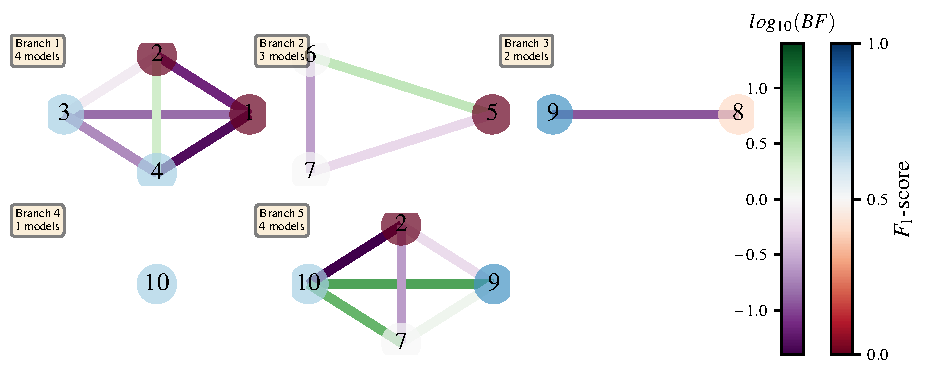
\includegraphics{qmla_run_data/Jan_18/18_04/instances/qmla_1/graphs_of_branches_ExampleGreedySearch.pdf}
    }
    \end{center}
    \caption[Greedy \glsentrylong{es}]{
        Greedy \glsentrylong{es}. 
        \textbf{(a)}, model compostion. 
        \textbf{b}, graph of branches on the \glsentrylong{et}. 
        Models are coloured by their $\fs$, and edges represent the \gls{bf} between models. 
        The first four branches are equivalent to those in \cref{fig:greedy_exploration_strategy} ,
        while the final branch considers the set of branch champions, in order to determine the overall champion. 
    }
    \label{fig:example_es_greedy}
\end{figure}


\subsection{Tiered greedy search}
We provide one final example of a non-trivial \gls{es}: 
    tiered greedy search. 
Similar to the idea of \cref{sec:greedy_search}, 
    except terms are introduced hierarchically:
    sets of terms $\termset_1, \termset_2, \dots \termset_n$ 
    are each examined greedily, where the overall strongest model of one tier 
    forms the seed model for the subsequent tier. 
This is depicted in the main text in \cref{fig:greedy_search}. 
A corresponding \gls{es} is given as follows. 

\begin{lstlisting}[
    label=listing:tiered_greedy_exploration_strategy,
    caption={\ttt{ExampleGreedySearchTiered} exploration stategy},
    language=Bash
]

class ExampleGreedySearchTiered(
    exploration_strategy.ExplorationStrategy
):
    r"""
    Greedy search in tiers.

    Terms are batched together in tiers; 
    tiers are searched greedily; 
    a single tier champion is elevated to the subsequent tier. 

    """

    def __init__(
        self,
        exploration_rules,
        **kwargs
    ):
        super().__init__(
            exploration_rules=exploration_rules,
            **kwargs
        )
        self.true_model = 'pauliSet_1_x_d3+pauliSet_1J2_yJy_d3+pauliSet_1J2J3_zJzJz_d3'
        self.initial_models = None
        self.term_tiers = {
            1 : ['pauliSet_1_x_d3', 'pauliSet_1_y_d3', 'pauliSet_1_z_d3' ],
            2 : ['pauliSet_1J2_xJx_d3', 'pauliSet_1J2_yJy_d3', 'pauliSet_1J2_zJz_d3'],
            3 : ['pauliSet_1J2J3_xJxJx_d3', 'pauliSet_1J2J3_yJyJy_d3', 'pauliSet_1J2J3_zJzJz_d3'],
        }
        self.tier = 1
        self.max_tier = max(self.term_tiers)
        self.tier_branch_champs = {k : [] for k in self.term_tiers} 
        self.tier_champs = {}
        self.prune_completed_initially = True
        self.check_champion_reducibility = True

    def generate_models(
        self,
        model_list,
        **kwargs
    ):
        self.log_print([
            "Generating models in tiered greedy search at spawn step {}.".format(
                self.spawn_step, 
            )
        ])

        if self.spawn_stage[-1] is None:
            try:
                previous_branch_champ = model_list[0]
                self.tier_branch_champs[self.tier].append(previous_branch_champ)
            except:
                previous_branch_champ = None

        elif "getting_tier_champ" in self.spawn_stage[-1]:
            previous_branch_champ = model_list[0]
            self.log_print([
                "Tier champ for {} is {}".format(self.tier, model_list[0])
            ])
            self.tier_champs[self.tier] = model_list[0]
            self.tier += 1
            self.log_print(["Tier now = ", self.tier])
            self.spawn_stage.append(None) # normal processing

            if self.tier > self.max_tier:
                self.log_print(["Completed tree for ES"])
                self.spawn_stage.append('Complete')
                return list(self.tier_champs.values())
        else:
            self.log_print([
                "Spawn stage:", self.spawn_stage
            ])

        new_models = greedy_add(
            current_model = previous_branch_champ, 
            terms = self.term_tiers[self.tier]
        )
        self.log_print([
            "tiered search new_models=", new_models
        ])

        if len(new_models) == 0:
            # no models left to find - get champions of branches from this tier
            new_models = self.tier_branch_champs[self.tier]
            self.log_print([
                "tier champions: {}".format(new_models)
            ])
            self.spawn_stage.append("getting_tier_champ_{}".format(self.tier))
        return new_models

def greedy_add(
    current_model, 
    terms,
):
    r""" 
    Combines given model with all terms from a set.
    
    Determines which terms are not yet present in the model, 
    and adds them each separately to the current model. 

    :param str current_model: base model
    :param list terms: list of strings of terms which are to be added greedily. 
    """

    try:
        present_terms = current_model.split('+')
    except:
        present_terms = []
    nonpresent_terms = list(set(terms) - set(present_terms))
    
    term_sets = [
        present_terms+[t] for t in nonpresent_terms
    ]

    new_models = ["+".join(term_set) for term_set in term_sets]
    
    return new_models
\end{lstlisting}

with corresponding results in \cref{fig:example_es_tiered_greedy}. 
\begin{figure}[H]
    \begin{center}
    \subfloat[]{
        \includegraphics{qmla_run_data/Jan_18/19_06/instances/qmla_1/composition_of_models.pdf}
    }
    \qquad
    \subfloat[]{
        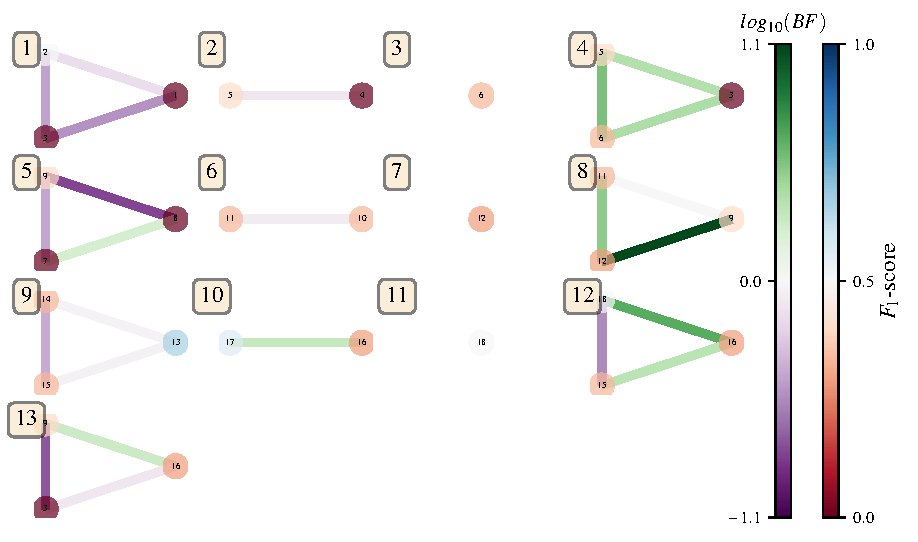
\includegraphics{qmla_run_data/Jan_18/19_06/instances/qmla_1/graphs_of_branches_ExampleGreedySearchTiered.pdf}
    }
    \end{center}
    \caption[Tiered greedy \glsentrylong{es}]{
        Tiered greedy \glsentrylong{es}. 
        \textbf{(a)}, \ttt{composition_of_models}. 
        \textbf{b}, \ttt{graphs_of_branches_ExampleGreedySearchTiered}: graph of branches on the \glsentrylong{et}. 
        Models are coloured by their $\fs$, and edges represent the \gls{bf} between models. 
        In each tier, three branches greedily add terms, and a fourth branch considers the champions of the first three branches
        in order to nominate a tier champion. 
        The final branch consists only of the tier champions, to nominate the global champion, $\hp$.  
    }
    \label{fig:example_es_tiered_greedy}
\end{figure}

